%! suppress = TooLargeSection
%! suppress = SentenceEndWithCapital
%! suppress = TooLargeSection
% Preamble
\documentclass[11pt]{PyRollDocs}
\usepackage{textcomp}
\usepackage{csquotes}
\usepackage{wasysym}

\addbibresource{refs.bib}
% Document
\begin{document}

    \title{Neutral Point Estimator PyRolL Plugin}
    \author{Christoph Renzing}
    \date{\today}

    \maketitle

    The PyRolL plugin pyroll-neutral-line-estimator provides different estimators for the neutral point which markes the point of zero shear stresses inside the roll gap.


    \section{Model approach}\label{sec:model-approach}

    For rolling in grooves as for flat rolling, the neutral point is the point inside the roll gap where the shear stresses become zero.
    Hence, rolling is a three-dimensional forming process, the neutral point isn't a point but a curved plane inside the roll gap.
    For flat rolling as for groove rolling, the actual plane is often assumed as a point marking the horizontal coordinate inside the roll gap.
    In the case of groove rolling, \textcite{Kunzman1977} stated that due to the spreading of the material the roll gap has to be divided into a forward-slip area, a backward-slip area
    as well as two areas which are called spreading areas.
    \autoref{fig:neutral-plane-groove-rolling} shows a simplified sketch of the areas during rolling.

    \begin{figure}
        \centering
        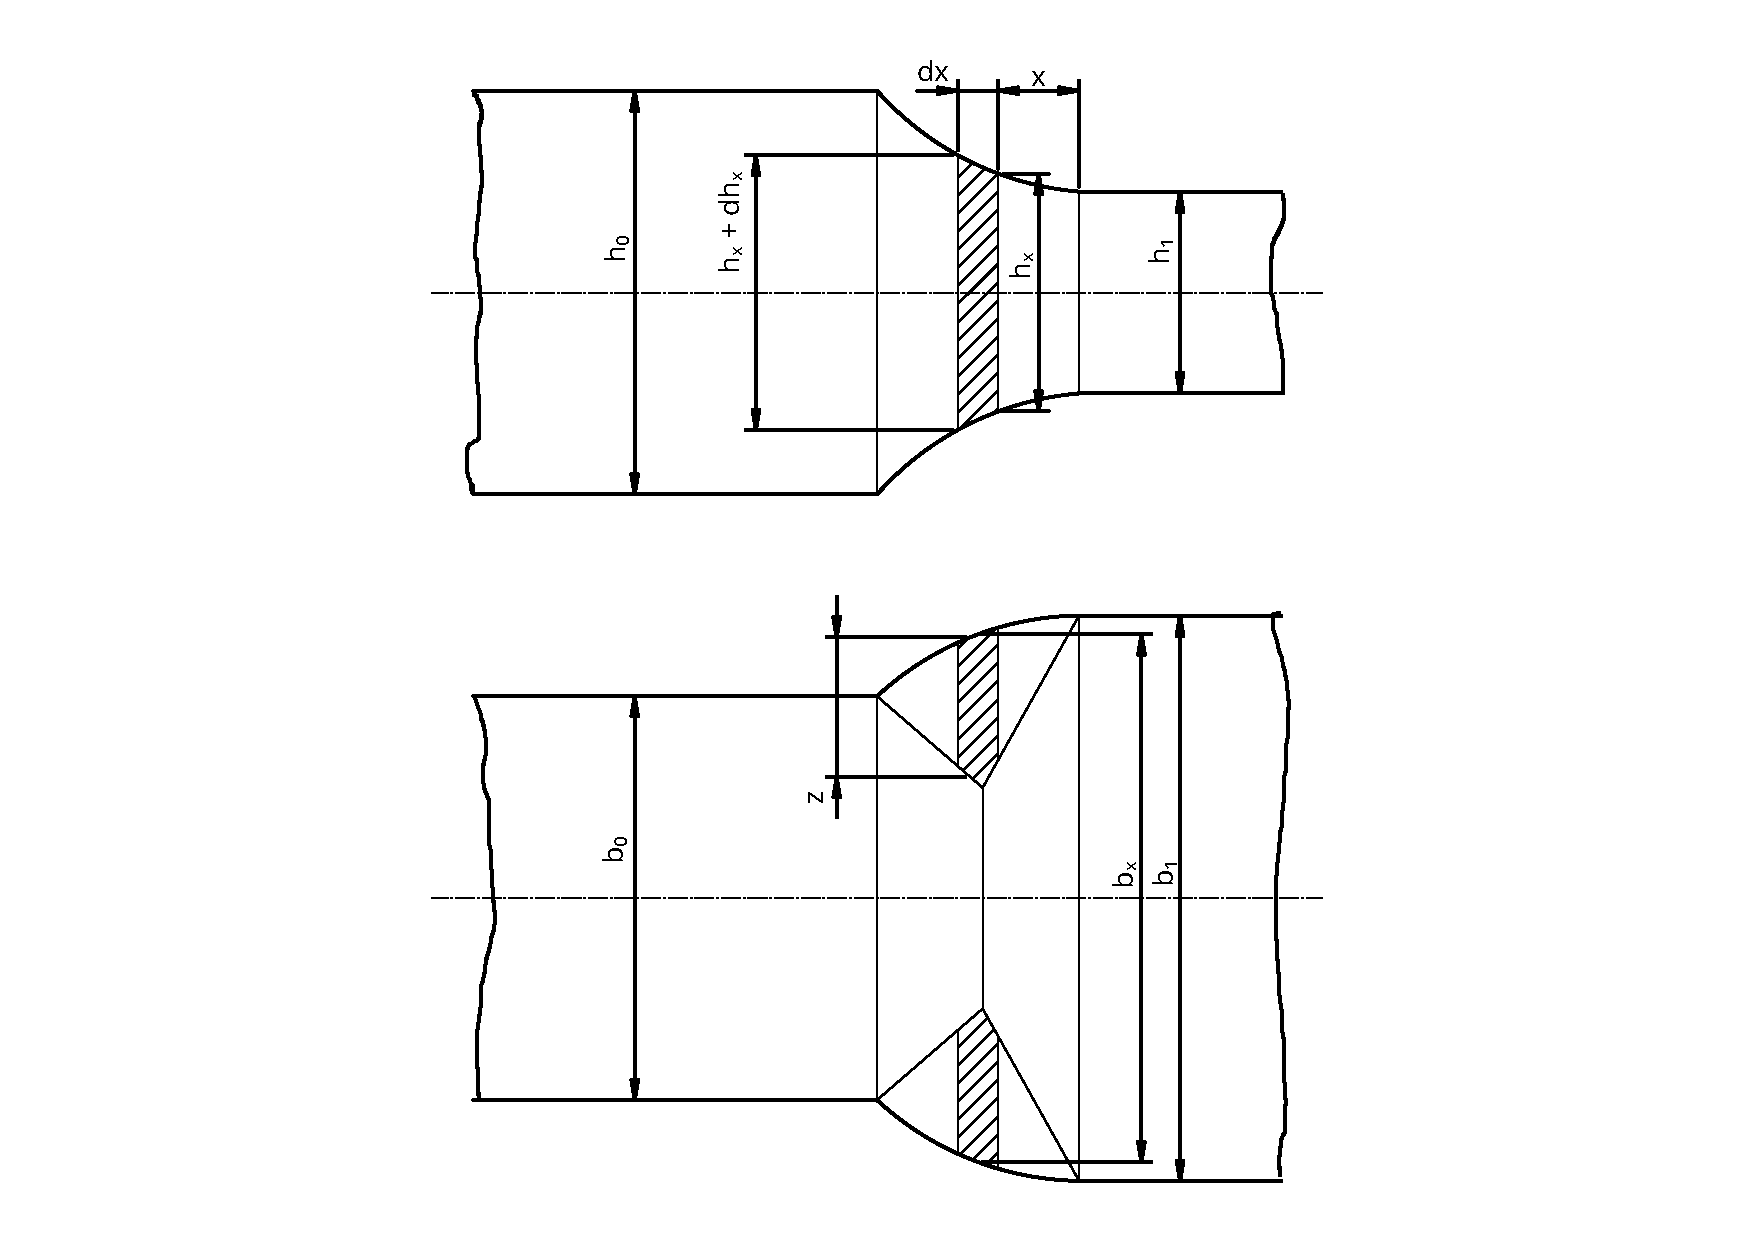
\includegraphics[width=0.8\textwidth]{img/kunzmann_neutral_plane}
        \caption{Neutral Plane for groove rolling}
        \label{fig:neutral-plane-groove-rolling}
    \end{figure}

    The pyroll-neutral-point-estimator plugin provides different simplified solutions derived by different authors for flat rolling.
    Featured model equations are taken from \textcite{Ford1951, Bland1948}, \textcite{Sims1954}, \textcite{Siebel1925} as well as \textcite{Bryant1973}.

    Since all of those solutions, derived from various simplified assumptions about the conditions inside the roll gap, are calculating the roll angle of the neutral point, the horizontal coordinate of the neutral point is calculated using equation~\ref{eq:angle-to-coordinate}.

    \begin{equation}
        x_n = -R_w \sin\left( \alpha_n \right)
        \label{eq:angle-to-coordinate}
    \end{equation}


    \section{Usage instructions}\label{sec:usage-instructions}
    The plugin can be loaded under the name \texttt{pyroll\_neutral\_point\_estimator}.

    An implementation of the \lstinline{neutral_point} hook on \lstinline{RollPass} is provided.
    Furthermore, to decide which estimator is used the \lstinline{pyroll.neutral_point_estimator.Config.ESTIMATOR} variable can be set according to table~\ref{tab:hookspecs}.

    \begin{table}
        \centering
        \caption{Config variables for different estimators.}
        \label{tab:hookspecs}
        \begin{tabular}{ll}
            \toprule
            Estimator                 & Variable Name              \\
            \midrule
            Equal Solution            & \enquote{EQUAL}            \\
            Ford-Ellis-Bland Solution & \enquote{FORD-ELLIS-BLAND} \\
            Sims Solution             & \enquote{SIMS}             \\
            Siebel Solution           & \enquote{SIEBEL}           \\
            Osborn Solution           & \enquote{OSBORN}           \\
            \bottomrule
        \end{tabular}
    \end{table}

    \printbibliography


\end{document}